
\section{Wireless Communication}

\begin{tabular}{|l|ccc|}
    \hline
    Classification & Mobile & Wireless Sensor Network & Internet Of Things\\
    \hline
    Network size & Millions & Thousand & Millions to Billions? \\
    Range & 100 to 1000$km^2$ & $m^2$ to $km^2$ & $m^2$ to $km^2$\\
    Mobility & Mobile & Static or mobile & Static or mobile \\
    Roaming & Yes & x & x \\
    Energy & Not critical & Critical & x \\
    Speed & Best without constraint & x & x \\
    \hline
\end{tabular}


\subsection{Radio spectrum}
Not all frequencies are equally suitable for all purpose
\begin{itemize}
    \item $\neq$ propagation properties
    \item $\neq$ power emission
    \item Some a reserved (police, phone) other are license free
\end{itemize}

\subsection{Path loss}

Signal strength is attenuated as the electromagnetic wave propagates
through space.

\subsubsection{Free-space loss}
Attenuation depends on frequency and distance
$$\frac{P_r}{P_t} = G_t \times G_r \times ( \frac{\lambda}{4\pi R})^2$$
where \begin{tabular}{rl}
    $P_r,P_t$ & is the received and transmitted power\\
    $G_r,G_t$ & is the received and transmitted antenna gain\\
    $R$ & is the distance between transmitter and receiver\\
    $\lambda$ & is the wave length\\
\end{tabular}

$$PL[dB] = 10 log\frac{P_t}{P_r} = - 10 log\frac{P_r}{P_t}$$

\subsubsection{Others loss}
\begin{center}
    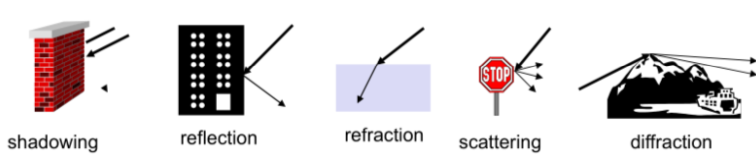
\includegraphics[width=0.7\linewidth]{img/loss.png}
\end{center}

\begin{itemize}
    \item Reflection and refraction depend on material and wave
        length
    \item Multi-path (scattering, diffraction,...)
        $$\frac{P_r}{P_t} = G_t \times G_r \times ( \frac{\lambda}{4\pi
        R})^\gamma$$
        where $\gamma$ is 3-5 in cities, 4-6 in buildings,...
    \item Noise due to
        \begin{itemize}
            \item Receiver electronics
            \item Interference on wireless channel:
                B far away to be detected by A, but still causes
                interference in form of background noise.
                \begin{center}
                    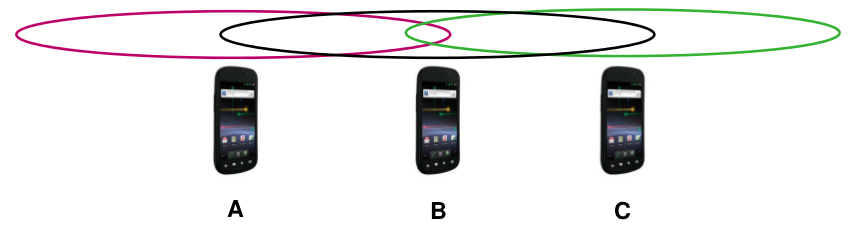
\includegraphics[width=0.5\linewidth]{img/ranges.png}
                \end{center}

                \paragraph{Hidden stations}: (1) C cannot detect A, (2) send data to B
                but (3) B cannot receive because A is sending
                \paragraph{Far stations}: (1) A is closer to B than C so
                (2) signal of A so strong that B cannot receive C
        \end{itemize}

        Stronger the noise, harder for the receiver to interpret signal
        as a symbol ($0-1$).
        \begin{itemize}
            \item Expressed as Signal-To-Noise: $$SNIR = 10 log(\frac{P_r}{N_0 + \sum_j I_j})$$ 
                where \begin{tabular}{rl} $P_r$ & Received signal power \\
                $N_0$ & Noise power \\
                $I_j$ & Influence of interfering neighbor $j$
            \end{tabular}

        \item With an appropriate Medium Access protocol (we will see
            that later), interference can be reduced. SNIR simplifies to
            SNR (Signal-Noise-Ratio)
            $$SNR=10 log(\frac{P_r}{P_N})$$
            where \begin{tabular}{rl} $P_r$ & Received signal power \\
            $P_N$ & noise power varies from locality\\
        \end{tabular}
\end{itemize}
\end{itemize}

\subsubsection{Error Rate} 
\begin{itemize}
    \item BER (Bit Error Rate): Number of bit errors per time unit
        $\Rightarrow$ depends on $SNR$

        $p_b$ is the probability that a received bit will be in error
    \item PER (Packet Error Rate): Packet rate error.
        $p_p$ is the probability that a received packet has an error
\end{itemize}

$$p_p = 1 - (1 - p_b)^N$$ where $N$ is the packet size


\subsection{Physical layer}

%\begin{center}
%    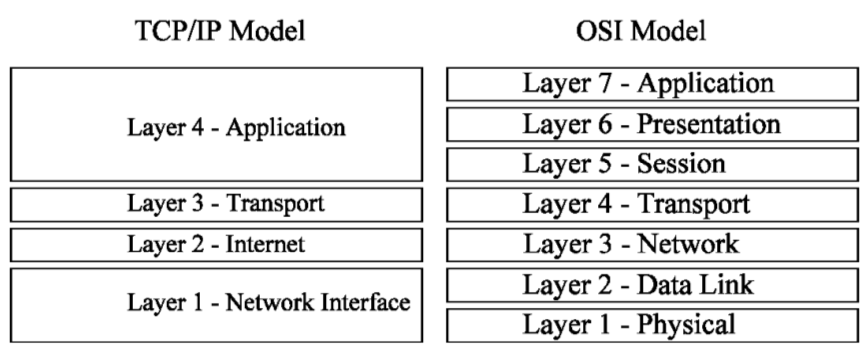
\includegraphics[width=0.6\linewidth]{img/osi.png}
%\end{center}
\begin{center}
    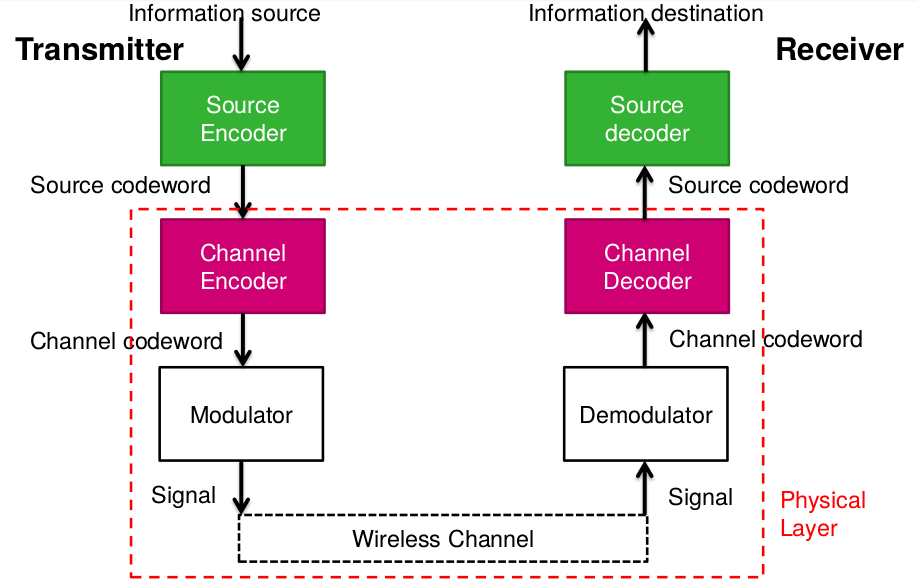
\includegraphics[width=0.8\linewidth]{img/physical.png}
\end{center}

\begin{itemize}
    \item \textbf{Source encoding}: also does compression based on
        information statistics, use fewer number of bits

    \item \textbf{Channel encoding}
        \begin{itemize}
            \item Add error detection code to the data (parity bits, CRC)
            \item Block coding 

            \item interleaving (shuffle symbols): As electromagnetic spikes can
                cause burst errors, many errors in one code word $\Rightarrow$
                exceeds error-correcting capabilities.

                Shuffle symbols to distribute error over several words: Hello
                World $\rightarrow$ HWeol rllod
        \end{itemize}
\end{itemize}

\subsubsection{Modulation}
Radio wave as sine function: $signal(t) = A \times sin(2\pi \times t
\times f + \phi)$ with Amplitude (A), Frequency (f) and Phase ($\phi$).


Modulation manipulates these parameters as a function of time to
transmit data.
\begin{center}
    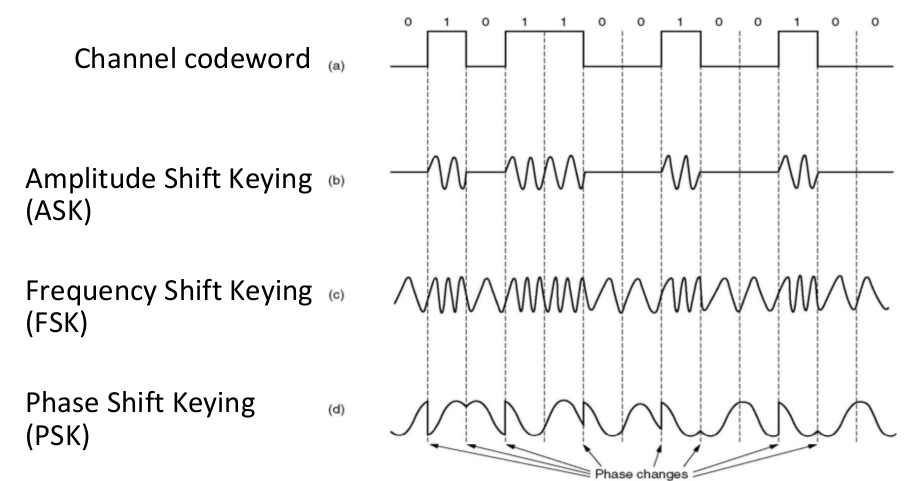
\includegraphics[width=0.6\linewidth]{img/modulation.png}
\end{center}

Challenge: bit synchronization, frame synchronization, listing same
frequency, noise, interference,...


